%!TEX root = ../report.tex

\begin{document}
    \chapter{Methodology}

    \section{Pipeline Workflow: 2D Binary Lane segmentation}
        \subsection{Architectural Overview}
        We first utilized the dual stage architecture proposed by \cite{guo2020gen} to obtain 3D lane points, where the output from the first stage is binary lane segmentation. And authors have not explored the efficacy of more complex architecture for binary 2D lane segmentation on 3D lane detection results. So we experimented with some mentioned approaches in section 3.1 for the same. In this section we will briefly discuss the neural network architecture for the binary 2D lane segmentation that we have experimented in this work. 
        
        Originally \cite{guo2020gen} have utilized ERFNet\cite{Romera2018ERFNetER} based network to obtain binary segmentation which is an auto-encoder based network for the first stage. For that we conducted a comaparative evaluation with the existing pretrained models using CondLaneNet\cite{DBLP:journals/corr/abs-2105-05003}, SCNN\cite{pan2018SCNN}, RESA\cite{DBLP:journals/corr/abs-2008-13719}, UFLD\cite{DBLP:journals/corr/abs-2004-11757}, LaneATT\cite{https://doi.org/10.48550/arxiv.2010.12035} which we will talk about in the later sections. As we have discussed in section 3.1 that there is more scope in extracting more meaningful features for segmentation based 2D lane detection and to facilitate the 3D lane detection we need 2D binary lane segmentation as an intermediate output. so explored two segmentation based approaches as mentioned above SCNN\cite{pan2018SCNN}, RESA\cite{DBLP:journals/corr/abs-2008-13719}. Both of these approaches are using semantic segmentation to predict 2D lane line points where the input to the network is a monocular image. But in out case we need binary segmentation as the output, so we modified the existing approaches to work for 2D binary lane segmentation.    
        
           \begin{figure}[h]
    \centering
    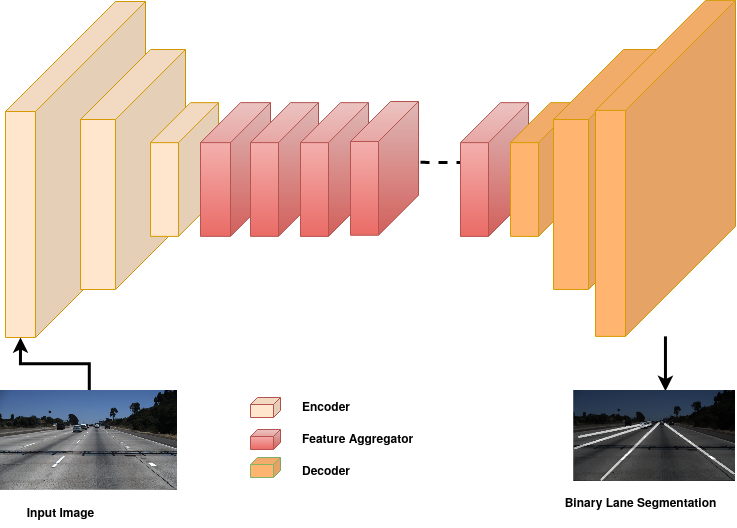
\includegraphics[width=12cm, height=7cm]{images/2dlane_pipleline.png}
    \caption{2D Binary Lane segmentation Pipeline}
    \end{figure}
        
        Figure 4.4 represents the pseudo architecture for the 2D binary lane detection module. This is an auto-encoder based pipeline where we have used \ResNet{DBLP:journals/corr/HeZRS15} based network for initial feature encoding and later utilizing the feature aggregation modules proposed by SCNN\cite{pan2018SCNN} and RESA\cite{DBLP:journals/corr/abs-2008-13719}. In the end we have experimented with two types of decoders for upsampling the extracted features as it is a dense prediction task we need the output to be of the same spatial size as input. Initially we used the a simple decoder propsed by \SCNN{pan2018SCNN} which uses bi-linear interpolation to upsample the feature maps, later we experimented with the Bilateral Upsampling Decoder (BUSD) proposed by RESA\cite{DBLP:journals/corr/abs-2008-13719}. So we trained our 2d binary lane segmentation pipeline using mix and match of the above mentioned modules. 
        
        
        \subsection{Datasets Used}
        We utilized two datasets for training the 2D binary lane segmentation pipeline. The first dataset we used is TuSimple lane detection benchmark\cite{Tusimple}, as discussed in section 3.3.3 it is a simple dataset consists of normal highway driving. On the other hand we also use a more complex and much larger dataset compared to the previous one like CULane\cite{pan2018SCNN} which contains 55 hours of driving and contains different driving scenarios as discussed in section 3.3.3.    
        
        \subsection{Evaluation Metrics}
        Both the utilized datasets have their own evaluation metrics and even the authors have released the script for bench-marking the results and the evaluation criteria proposed by them only relies on penalizing the predictions on the basis of predicted 2d lane line points. As in our case we are not interested in predicting lane line points rather our 3D lane detection module relies on 2d binary lane segmentation masks as intermediate output. So we have used IoU (Intersection-over-union) or Jaccard Index to evaluate the trained models. IoU is a commonly used evaluation metric for image segmentation which is really effective. In Simple terms IoU calculated the area of overlap between the predicted segmentation mask and the ground truth divided by the union of the predicted segmentation mask and ground truth.
        
         \begin{figure}[h]
    \centering
    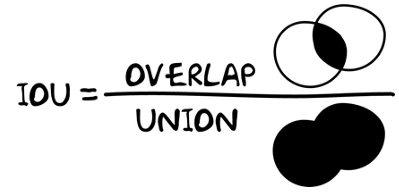
\includegraphics[width=7cm, height=4cm]{images/IOU.png}
    \caption{(IoU)Intersection-Over-Union \footnotemark}
    \end{figure}
    \footnotetext{\url{https://towardsdatascience.com/intersection-over-union-iou-calculation-for-evaluating-an-image-segmentation-model-8b22e2e84686}}
        
        \subsection{Implementation Details}
        \textbf{<TO BE FILLED LATER, talk about the image resize, hyper parameter used>}
        
    %---------------------------------------------------------------- After here must start 3d lane detection section%   
        
        \section{Pipeline Workflow: 3D Lane Detection }
        
        \subsection{3D Lane Geometry}
        In this section we will introduce the geometric representation of lanes in 3D space, image plane and birds eye view via the means of the transformation from one space to another. 
        
         \begin{figure}[h]
    \centering
    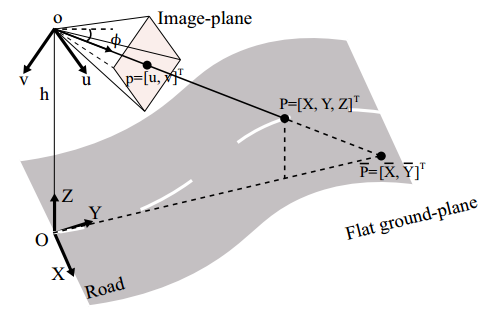
\includegraphics[width=9cm, height=5cm]{images/3d_lane_geometry.png}
    \caption{Geometric representation of lane point in 3D world space, image plane and virtual top view \cite{DBLP:journals/corr/abs-2112-15351}}
    \end{figure}
    
    In the above figure the point $\textbf{P} =[X, Y, Z]^{T}$ is in 3D space and when it is projected onto the image plane it is defined by $\textbf{p} = [u, v]^{T}$. Birds eye view can be seen as the projection of point $\textbf{P}$ from 3D space to flat ground plane, where $Z=0$. $\textbf{O}$ is the origin of the 3D space which is obtained by projecting the origin of camera center $\textbf{o}$ on to the flat ground plane with $Z = 0$. The focal length and other intrinsic parameters of the camera is fixed, where as the orientation of the camera in terms of camera height \textbf{h}  and camera pitch \textbf{$\phi$} is fixed or sometimes it is predicted from the network. 
    
    Using geometric transformation and homography as discussed above we can project points in 3D space to virtual flat ground plane. As per the figure 4.1 we can say that the point \textbf{P} it projection on image plane and flat ground plane, all lies on the same ray and this co-linear relationship will hold even if when there are downhill scenarios where $Z<0$. 
    
      \begin{figure}[h]
    \centering
    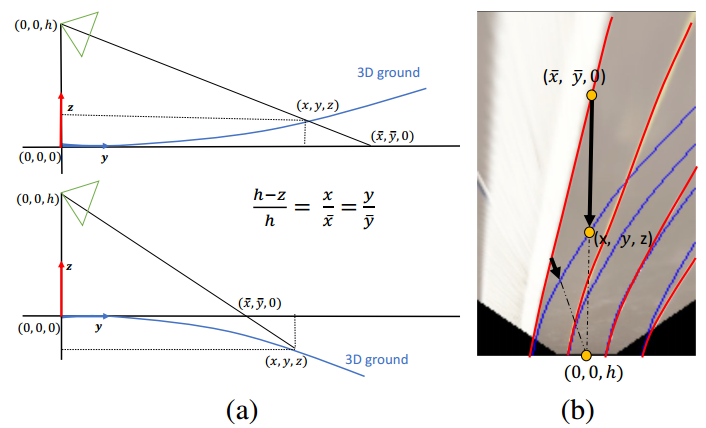
\includegraphics[width=9cm, height=5cm]{images/collinear_3dlane.png}
    \caption{Another view of the co-linear relationship between the 3D lane points $(x,y,z)$, its projection on virtual top view $(\overline{x}, \overline{y},0)$ and camera center $(0,0,h)$ \cite{guo2020gen}}
    \end{figure}

    Therefore we can obtain a relationship between the points from 3d world to virtual top view as :
    \begin{center}
        $\frac{h-z}{h} =\frac{x}{\overline{x}}=\frac{y}{\overline{y}}$ 
    \end{center}
    
    using the above formulation we can represent this transformation from 3D world space to virtual top view as \textbf{$\overline{P} = GP$}, where \textbf{G} is the transformation matrix. Similarly a point \textbf{$\overline{P}$} can be projected onto the image plane as $\textbf{p}$ using homomgraphy which is also discussed in section 2.2. and this can be represented as: 
    \begin{center}
       $\begin{bmatrix}\overline{u}  \\\overline{v} \\ \overline{z}\end{bmatrix} = \begin{bmatrix} f_{x} & 0& c_{x}  \\0 &f_{x} & c_{y} \\ 0 & 0 & 1     \end{bmatrix}\begin{bmatrix} 1 & 0& 0  \\0 &cos(\phi+ \frac{\theta}{2}) & h \\ 0 &cos(\phi+ \frac{\theta}{2}) & 0     \end{bmatrix}\begin{bmatrix}\overline{X}  \\\overline{Y} \\ 1\end{bmatrix}$
    \end{center}

    Here, \textbf{$\widetilde{p}$} $= (\widetilde{u}, \widetilde{v}, \widetilde{z})$ and  \textbf{$\widetilde{P}$} $= (\overline{X},\overline{Y},1 )$ are represented in the form of homogeneous coordinates, therefore $u = \frac{\widetilde{u}} {\widetilde{z}} $ and $v = \frac{\widetilde{v}} {\widetilde{z}} $. Similar as above this can be represented as \textbf{$\widetilde{p} = H\widetilde{P}$}, where H is the homography transformation matrix. 
    
    \subsection{3D Lane Anchor Representation}
    Some of the approaches used in this work are predicting 3D lane line points in the from of anchors and even the ground-truth points are also converted in the form of anchors as target tensors to the network.  As per the 3D lane geometry discussed above, x is the lateral axes and Y is the forward axes with respect to a scene. These anchors are generally predefined on the basis of  equally spaced distance in x and y directions. 
    
     \begin{figure}[h]
    \centering
    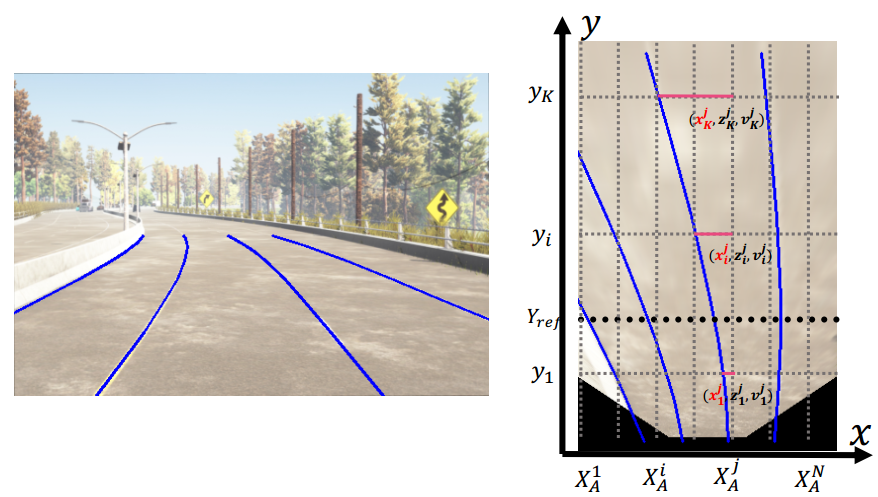
\includegraphics[width=9cm, height=5cm]{images/anchor_3Dlane.png}
    \caption{Lane anchor representation \cite{guo2020gen}}
    \end{figure}
    
    As per the figure 4.3, there exist N lane anchors (Vertical lines) in terms of N equally spaced position in X-direction ($X^{i}_{A}$)$^{N}_{i=1}$. The position on anchors in y-direction can be equally spaced or on the basis of certain distances in the forward direction. Therefore a 3D lane line in this can be represented by an anchor $X^{i}_{A}$ where each anchor contains $3*K$ attributes. K is the number of steps in y-direction. So at each step $(Y_ref)$ ground-truth lane anchor attributes ($\overline{x}^{i}_{j},z^{i}_{j},v^{i}_{j}$)$^{K}_{j=1}$ are calculated by associating it with the closest distance in x-direction. $\overline{x}^{i}_{j}$ are the horizontal offsets, $v^{i}_{j}$ is the visibility vector for every lane point.  In the later sections we will talk about the approaches that we have experimented with to obtain 3D lane line points. 
        
        \subsection{Architectural Overview: GenLaneNet\cite{guo2020gen}}
        
        Initially we have utilized the dual stage architecture proposed by \cite{guo2020gen} to obtain 3D lane points and later this dual stage way of architecture is used in our proposed 3D lane detection pipeline. In this section we will introduce the network architecture proposed by GenLaneNet\cite{guo2020gen} in detail and explain how we have utilized it for our initial experimentation for obtaining 3D lane line points.
        
         \begin{figure}[h]
    \centering
    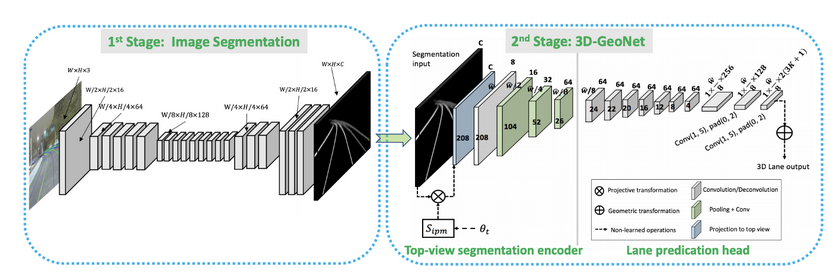
\includegraphics[width=13cm]{images/GenLaneNET.png}
    \caption{Network architecture of Gen-LaneNet \cite{guo2020gen}}
    \end{figure}
         
         Here authors have represented the 3D lane lines in the form of anchors and have utilized this representation to predict 3D lane line points by using a dual stage network. Authors have chosen this dual pathway approach on the fact that encoding 3D lane geometry is a different task to encoding features from image.
         The first stage is responsible for extracting features from the input monocular image and perform binary segmentation task on the image to obtain binary lane segmentation mask. This obtained binary lane segmentation mask is this used as an input for the next stage of the pipeline which is responsible for predicting the 3D lane line points in the form of anchor based representation. As described in section 4.2.2 each anchor defines a 3D lane line by 3*K values as ($\overline{x}^{i}_{j},z^{i}_{j},v^{i}_{j}$)$^{K}_{j=1}$. The ground truth target lane anchors are generated by taking the 3D lane line points which are in ego vehicle coordinate frame to virtual top view. 
         
         The output from the image segmentation stage is processed by a top view segmentation encoder which uses projective transformation and project it into top-view which are further processed by a series of convolution layers to encode features from top view binary segmentation. After that a lane prediction head predicts 3D lane line points in terms of anchor representation. The predicted anchors are in top-view which can be further transformed into 3D lane line points in ego-vehicle frame by using geometric transformation. This dual stage network makes the pipeline flexible in terms of using complex binary segmentation solutions and make it affordable as we don't need more real world 3D lane lines labels in various driving scenarios. Despite 
        
        \subsection{Proposed Architecture: 3D Lane Detection}
        
        Anchor based 3D lane detection approaches face similar challenges as anchor based 2D lane detection. Therefore it is not able to generalize well with different lane topologies. Utilizing the idea of dual stage network proposed by \cite{guo2020gen} and anchors less semi-local 3D lane detection approach proposed by \cite{}, we proposed an semi-local anchor-less dual stage network for obtaining 3D lane line points.
        
        \begin{figure}[h]
    \centering
    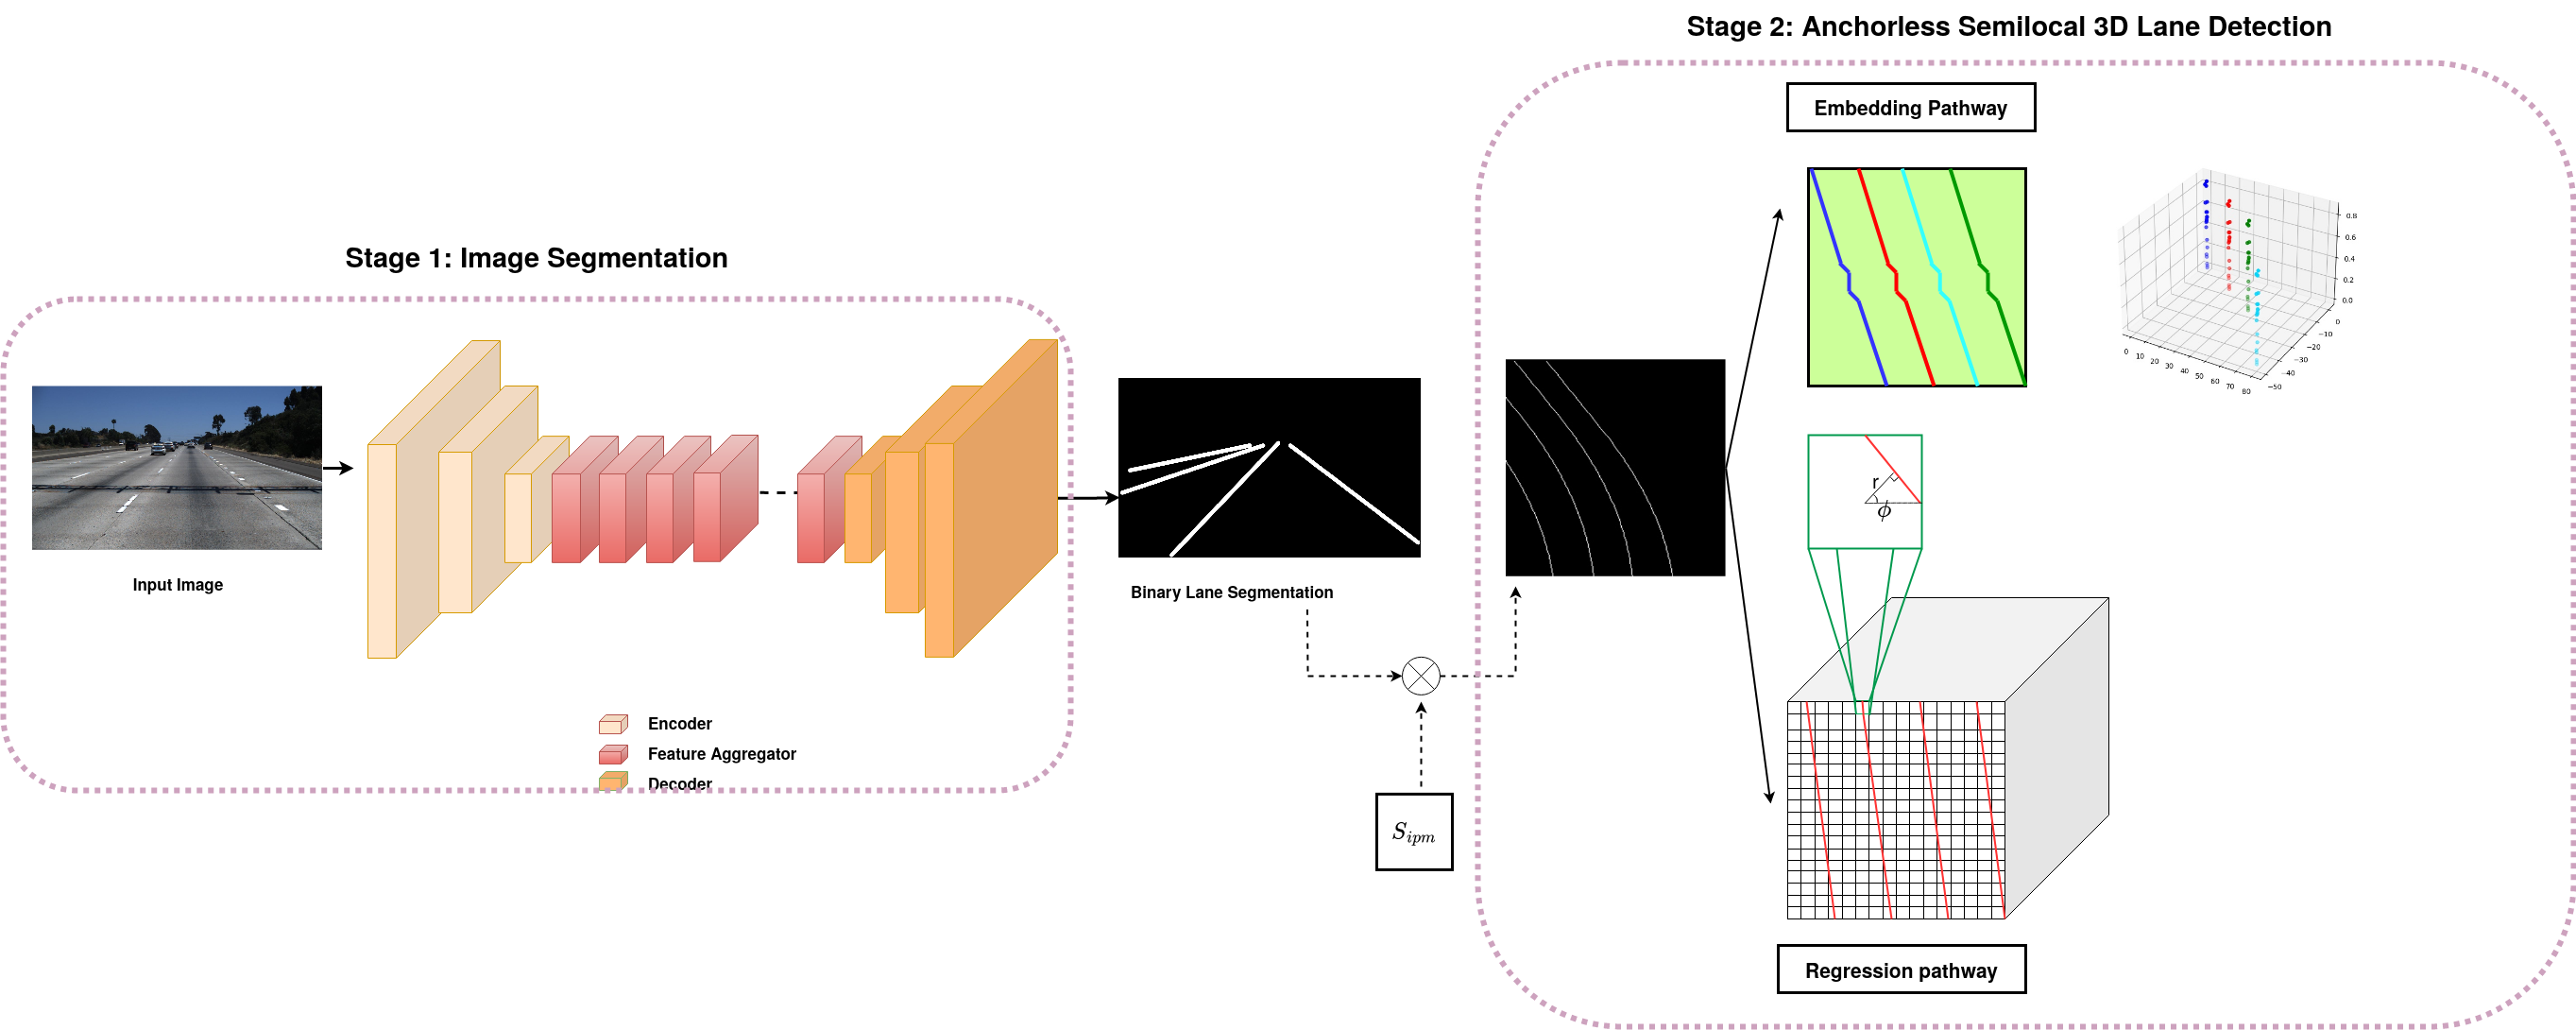
\includegraphics[width=\textwidth, height=7cm]{images/3DlaneAUXNet.png}
    \caption{Lane anchor representation \cite{guo2020gen}}
    \end{figure}
        
        
        \subsubsection{Stage 1: Image Segmentation}
        \subsubsection{Stage 2: Semi-Local 3D Lane Detection}
    
    \subsection{Loss Functions}
        (Write in general mentioning the sections which loss functions is used for what)
        
    \subsection{Experimental setup}
        \subsubsection{Datasets Used}
        \subsubsection{Evaluation Metrics}
        \subsubsection{Implementation Details}
    
    \section{Pipeline Workflow: 3D Lane AuxNet}
        \subsection{Architecture}
        \subsection{Dataset Used}
        \subsection{Evaluation Metrics}
        \subsection{Implementation Details}
        
\end{document}
